%\documentclass[paper=a4, fontsize=9pt]{article} 
\documentclass[a4paper,twoside,10pt]{amsart}


%\usepackage[scale=0.8]{geometry}
\usepackage{fullpage}

\usepackage[T1]{fontenc} % Use 8-bit encoding that has 256 glyphs
\usepackage[english]{babel} % English language/hyphenation
\usepackage{amsmath,amsfonts,amsthm} % Math packages
\usepackage{xcolor}
\usepackage{hyperref}
\usepackage{tcolorbox}

\usepackage{tikz}
\usepackage{tkz-graph}

\numberwithin{equation}{section} % Number equations within sections (i.e. 1.1, 1.2, 2.1, 2.2 instead of 1, 2, 3, 4)
\numberwithin{figure}{section} % Number figures within sections (i.e. 1.1, 1.2, 2.1, 2.2 instead of 1, 2, 3, 4)
\numberwithin{table}{section} % Number tables within sections (i.e. 1.1, 1.2, 2.1, 2.2 instead of 1, 2, 3, 4)
\usepackage{graphicx}
\usepackage{caption}
\usepackage{subcaption}


\newcommand{\horrule}[1]{\rule{\linewidth}{#1}} % Create horizontal rule command with 1 argument of height
\newcommand{\ans}[1]{ { \color{gray} \itshape  #1} } % Create horizontal rule command with 1 argument of height

\newtheorem{theo}{Theorem}
\newtheorem{lemma}{Lemma}
\theoremstyle{definition}
\newtheorem{q_td}{Exercise }
\newcommand{\reftd}[1]{  $\circ$ \ref{#1}}
\newtheorem{q_tp}{$\diamond$}
\newcommand{\reftp}[1]{$\diamond$ \ref{#1}}

\begin{document}

%----------------------------------------------------------------------------------------
%	TITLE 
%----------------------------------------------------------------------------------------


\normalfont \normalsize 
\noindent\textsc{\small Universit\'e Grenoble Alpes  }\\
\noindent\textsc{\small  \hfill MSIAM 1st year} \\ [0.3cm] % Your university, school and/or department name(s)
\horrule{0.5pt} \\[0.4cm] % Thin top horizontal rule
\begin{center}
{\LARGE \scshape  Numerical Optimization\\ Tuto 1: Gradients and Minimization} \\ % The  title
\end{center}
\noindent\textsc{\hfill L. Desbat \& F. Iutzeler } 
\horrule{2pt} \\[0.5cm] % Thick bottom horizontal rule



%----------------------------------------------------------------------------------------
%	TD
%----------------------------------------------------------------------------------------
%\newpage
\setcounter{section}{0}
\renewcommand{\thesection}{\Alph{section}} 
\renewcommand*{\theHsection}{TD.\the\value{section}}


\vspace*{0.5cm}

\section{Differentiability, Minima, and Convexity}


\begin{q_td}[Quadratic functions]\label{td:qp}\hfill

\begin{itemize}
\item[a.] In $\mathbb{R}^n$, compute the gradient of the squared Euclidean norm $\|\cdot\|_2^2$ at a generic point $x\in\mathbb{R}^n$.
\item[b.] Let $A$ be an $m \times n$ real matrix and $b$ a size-$m$ real vector. We define $f(x) = \|Ax-b\|_2^2$. For a generic vector $a\in \mathbb{R}^n$, compute the gradient $\nabla f(a)$ and Hessian $H_f(a)$.
\item[c.] Let $C$ be an $n \times n$ real matrix, $d$ a size-$n$ real vector, and $e\in\mathbb{R}$. We define $g(x) = x^\mathrm{T}Cx + d^\mathrm{T}x + e$. For a generic vector $a\in \mathbb{R}^n$, compute the gradient $\nabla g(a)$ and Hessian $H_g(a)$.
\item[d.] Can all functions of the form of $f$ and be written in the form of $g$? And conversely? 
\end{itemize}
\end{q_td}


\vspace*{0.5cm}

\begin{q_td}[Basic Differential calculus]
\label{td:conv}
Use the composition lemma to compute the gradients of:
\begin{itemize}
\item[a.] $f_1(x) = \|Ax-b\|_2^2$  .
\item[b.] $f_2(x) = \|x\|_2$ .
\end{itemize}
\end{q_td}


\vspace*{0.5cm}

\begin{q_td}[Preparing the Lab]
\label{td:fun}
In the first lab, we will consider the following toy functions:
\begin{align*}
& \begin{array}{rrcll}
f: & \mathbb{R}^2 & \to &\mathbb{R}\\
& (x_1,x_2) & \mapsto  & 4 (x_1-3)^2 + 2(x_2-1)^2
\end{array}\\
%
& \begin{array}{rrcll}
g: & \mathbb{R}^2 & \to &\mathbb{R}\\
& (x_1,x_2) & \mapsto  & \log( 1 + \exp(4 (x_1-3)^2 ) + \exp( 2(x_2-1)^2 ) ) - \log(3)
\end{array} \\
%
& \begin{array}{rrcll}
r: & \mathbb{R}^2 & \to &\mathbb{R}\\
& (x_1,x_2) & \mapsto  &  (1-x_1)^2 + 100(x_2-x_1^2)^2
\end{array}\\
%
& \begin{array}{rrcll}
t: & \mathbb{R}^2 & \to &\mathbb{R}\\
& (x_1,x_2) & \mapsto  & (0.6 x_1 + 0.2 x_2)^2 \left((0.6 x_1 + 0.2 x_2)^2 - 4 (0.6 x_1 + 0.2 x_2)+4\right) + (-0.2 x_1 + 0.6 x_2)^2
\end{array}\\
%
& \begin{array}{rrcll}
p: & \mathbb{R}^2 & \to &\mathbb{R}\\
& (x_1,x_2) & \mapsto  &  \left| x_1-3 \right|  + 2\left| x_2-1\right| .
\end{array}
\end{align*}
\begin{itemize}
\item[a.] From the 3D plots of \ref{fig:3d}, which functions are visibly non-convex.
\item[b.] For all five functions, show that they are convex or give an argument for their non-convexity.
\item[c.] For functions $f,g,r,t$, compute their gradient.
\item[d.] For functions $f,g$, compute their Hessian.
\end{itemize}
\end{q_td}



\begin{figure}[h!]
    \centering
    \begin{subfigure}[b]{0.48\textwidth}
        \centering
        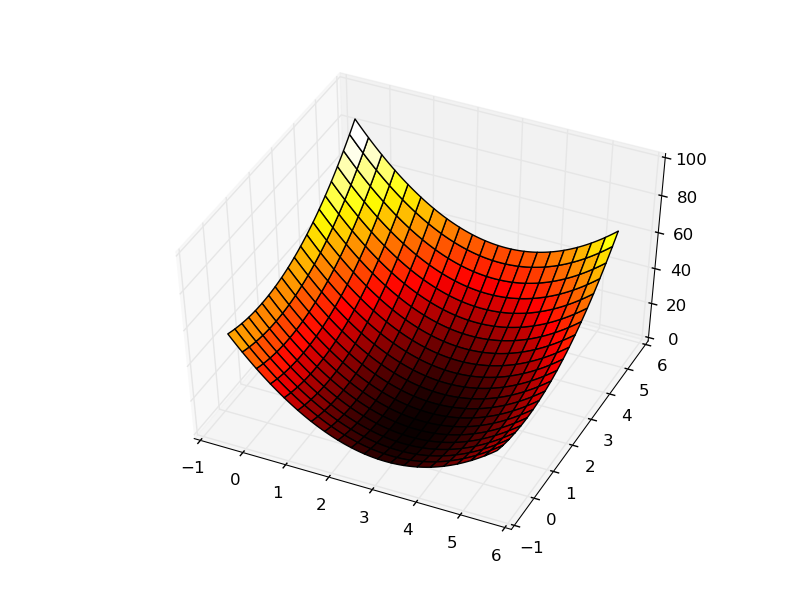
\includegraphics[width=1.0\textwidth]{simple.png}
        \caption{a \emph{simple} function: $f$}
    \end{subfigure}
    ~ 
    \begin{subfigure}[b]{0.48\textwidth}
        \centering
        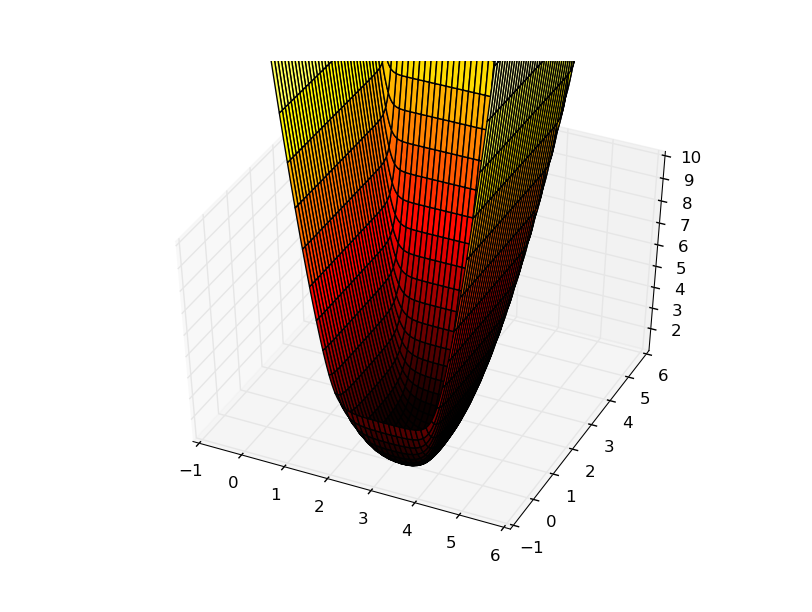
\includegraphics[width=1.0\textwidth]{harder.png}
        \caption{some \emph{harder} function: $g$}
    \end{subfigure} \\
    \centering
    \begin{subfigure}[b]{0.48\textwidth}
        \centering
        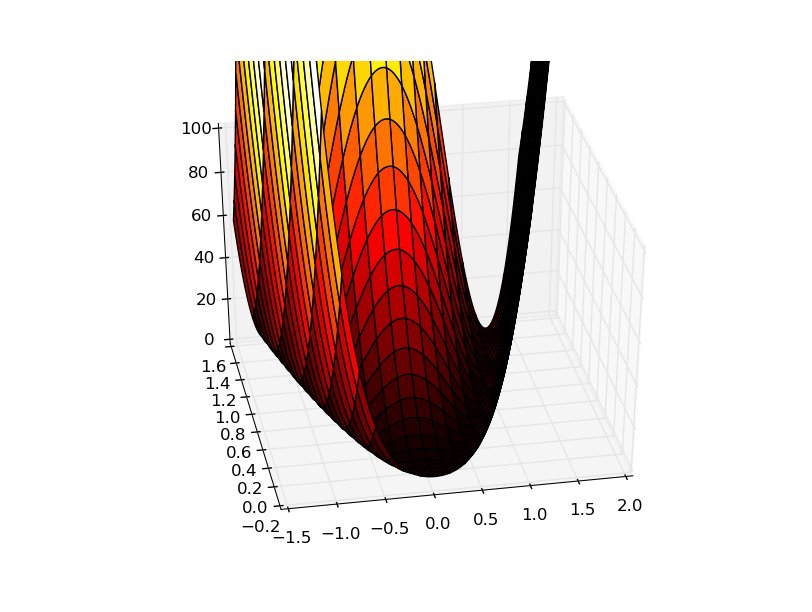
\includegraphics[width=1.0\textwidth]{rosenbrock.png}
        \caption{\emph{Rosenbrock}'s function: $r$}
    \end{subfigure}
    ~ 
    \begin{subfigure}[b]{0.48\textwidth}
        \centering
        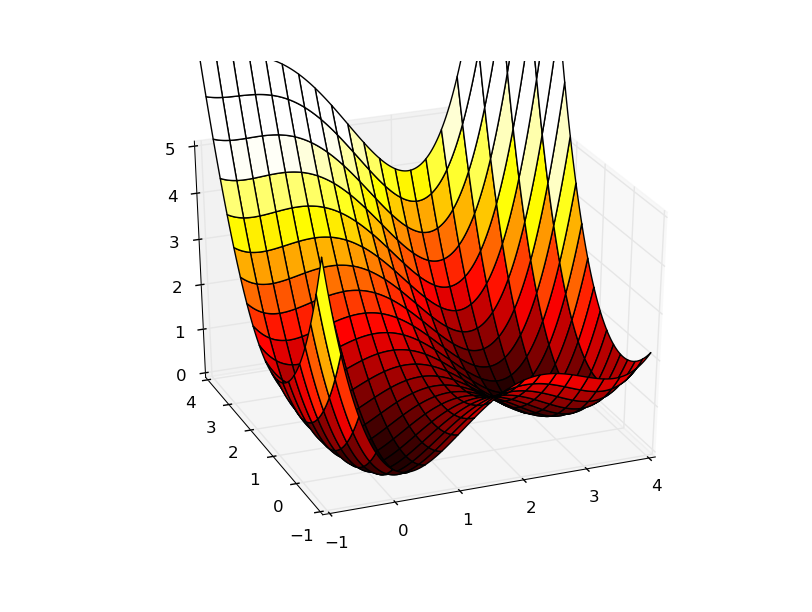
\includegraphics[width=1.0\textwidth]{two_pits.png}
        \caption{\emph{two pits} function: $t$}
    \end{subfigure}
    ~ 
    \begin{subfigure}[b]{0.48\textwidth}
        \centering
        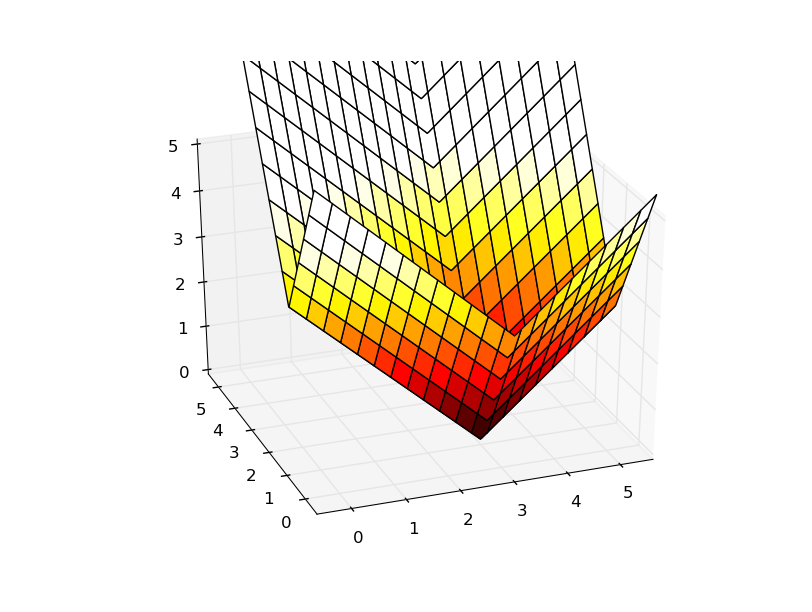
\includegraphics[width=1.0\textwidth]{poly.png}
        \caption{\emph{polyhedral} function: $p$}
    \end{subfigure}
    \caption{3D plots of the considered functions}
	\label{fig:3d}
\end{figure}



\vspace*{0.5cm}

\begin{q_td}[Fundamentals of convexity]
\label{td:conv}
~
\begin{itemize}
\item[a.] Let $f$ and $g$ be two convex functions. Show that $m(x) = \max(f(x),g(x) )$ is convex.
\item[b.] Show that $f_1(x) = \max(x^2-1 , 0)$ is convex. 
\item[c.] Let $f$ be a convex function and $g$ be a convex, non-decreasing function. Show that $c(x) = g(f(x))$ is convex.
\item[d.] Show that $f_2(x) =  \exp(x^2)$ is convex. What about $f_3(x) =  \exp(-x^2)$ 
\item[e.] Justify why the $1$-norm, the $2$ norm, and the squared $2$-norm are convex.
\end{itemize}
\end{q_td}

\vspace*{0.5cm}

\begin{q_td}[Strict and strong convexity]
\label{td:qp} A function $f:\mathbb{R}^n \to \mathbb{R}$ is said
\begin{itemize}
\item \emph{strictly convex} if for any $x \neq y \in\mathbb{R}^n$ and any $\alpha\in]0,1[$
$$ f(\alpha x + (1- \alpha )y ) < \alpha f(x) + (1- \alpha )f(y) $$
\item \emph{strongly convex} if there exists $\beta>0$ such that $f - \frac{\beta}{2}\|\cdot\|_2^2$ is convex.
\end{itemize}
\begin{itemize}
\item[a.] For a strictly convex function $f$, show that the problem
$$ \left\{ \begin{array}{l} \min f(x) \\ x \in C \end{array} \right. $$
where $C$ is a convex set admits at most one solution.
\item[b.] Show that a strongly convex function is also strictly convex.\\ \emph{(hint: use the identity $\|\alpha x + (1-\alpha)y\|^2 = \alpha \|x\|^2 + (1-\alpha)\|y\|^2 - \alpha (1-\alpha)\|x-y\|^2 $.)}
\end{itemize}
\end{q_td}

\vspace*{0.5cm}


\begin{q_td}[Optimality conditions]
\label{td:opt}
Let $f:\mathbb{R}^n\to\mathbb{R}$ be a twice differentiable function and $\bar{x}\in\mathbb{R}^n$. We suppose that $f$ admits a local minimum at $\bar{x}$ that is $f(x)\geq f(\bar{x})$ for all $x$ in a neighborhood\footnote{Formally, one would write $\forall x \in \mathbb{R}^n$ such that $\|x-\bar{x}\|\leq \varepsilon$ for $\varepsilon>0$ and some norm $\|\cdot\|$. } of $\bar{x}$.
\begin{itemize}
\item[a.] For any direction $u\in\mathbb{R}^n$, we define the $\mathbb{R}\to\mathbb{R}$ function $q(t) = f(\bar{x}+tu)$. Compute $q'(t)$.
\item[b.] By using the first order Taylor expansion of $q$ at $0$, show that $\nabla f(\bar{x}) = 0$.
\item[c.] Compute $q''(t)$. By using the second order Taylor expansion of $q$ at $0$, show that $\nabla^2 f(\bar{x})$ is positive semi-definite.
\end{itemize}
\end{q_td}

\vspace*{1cm}




\section{the Gradient Algorithm}

\begin{q_td}[Descent lemma]
\label{td:smooth}
A function $f:\mathbb{R}^n\to\mathbb{R}$ is said to be $L$-smooth if it is differentiable and  its gradient $\nabla f$ is $L$-Lipchitz continuous, that is
$$\forall x,y\in\mathbb{R}^n, ~~  \|\nabla f(x) - \nabla f(y) \| \leq L \|x-y\|. $$ 
The goal of the exercise is to prove that if $f:\mathbb{R}^n\to\mathbb{R}$ is $L$-smooth, then for all $x,y\in\mathbb{R}^n$,
$$ f(x) \leq f(y) +  (x-y)^\mathrm{T} \nabla f(y)  + \frac{L}{2} \| x-y\|^2 $$
\begin{itemize}
\item[a.] Starting from fundamental theorem of calculus stating that for all $x,y\in\mathbb{R}^n$,
$$ f(x) - f(y) = \int_{0}^1  (x-y)^\mathrm{T} \nabla f(y + t(x-y) ) \mathrm{d}t $$
prove the descent lemma.
\item[b.] Give a function for which the inequality is tight and one for which it is not.
\end{itemize}
\end{q_td}

\vspace*{0.5cm}

\begin{q_td}[Smooth functions]
Consider the constant stepsize gradient algorithm $x_{k+1} = x_k - \gamma \nabla f(x_k)$ on an $L$-smooth function $f$ with some minimizer (i.e. some $x^\star$ such that $f(x)\geq f(x^\star)$ for all $x$). 
\begin{itemize}
\item[a.] Use the \emph{descent lemma} to prove convergence of the sequence $(f(x_k))_k$ when $\gamma\leq 2/L$.
\item[b.] Did you use at some point that the function was convex? Conclude about the convergence of the gradient algorithm on smooth non-convex functions.
\end{itemize}
\end{q_td}







\end{document}
